\documentclass[]{article}

\usepackage{amsmath}
\usepackage{amsfonts}
\usepackage{amssymb}
\usepackage{xcolor}
\usepackage{url}
\usepackage{graphicx}
\usepackage{geometry}
\usepackage[most]{tcolorbox}

% {Begin zh_TW}
\usepackage{fontspec}   % 加這個就可以設定字體
\usepackage{xeCJK}       % 讓中英文字體分開設置
\setCJKmainfont{微軟正黑體} % 設定中文為系統上的字型,而英文不去更動,使用原 TeX 字型
\XeTeXlinebreaklocale "zh"             % 這兩行一定要加,中文才能自動換行
\XeTeXlinebreakskip = 0pt plus 1pt     % 這兩行一定要加,中文才能自動換行

\defaultCJKfontfeatures{AutoFakeBold=6,AutoFakeSlant=.4} %以後不用再設定粗斜
% {End zh_TW}

\setlength{\parindent}{0em}
\setlength{\parskip}{3ex}
\geometry{left=3cm, top = 3cm, right = 3cm, bottom = 3cm}

\newcommand{\ignore}[1]{}
\newcommand{\codequote}[1]{\colorbox{lightgray}{\tt #1}}

\begin{document}

\author{}  \date{}
\title{第 0 課:開始本課程之前}
\maketitle

\vspace{-4em}
-----------------

\section*{目標}

\begin{description}
	\item[---] 說明本課程的方法、大綱和目標聽眾
	\item[---] 詳述完成本課程所需的基本電腦能力
	\item[---] 提供一些關於如何完成這門課程的建議(應該對那些想嘗試的人有所幫助)
\end{description}

學完本課,你將能夠
\begin{description}
	\item[*] 決定是否開始學習這門課程
	\item[*] 確保你擁有所需的基本能力
\end{description}

\section*{目標聽眾和教學理念}

本課是針對沒有任何程式設計經驗的人。它還旨在合宜於那些不確定程式設計是否適合他們的人:他們可能對電腦感到有點害怕,或者他們可能已在第一門程式設計課程中失去了信心。

我們的理念可以概括為以下口號:\emph{小步走,不留空隙,一切都有意義}。我們相信程式設計就像學習一門新語言一樣容易---對某些人來說很難,對所有人來說都應是可行的\footnote{也就是說,除了極少數嚴重殘疾的。}。這需要一些努力和堅持,僅此而已。當然,有些人會比其他人做得更快。那又如何?

讓我們稍微解說一下口號,這也讓我們有機會說明清楚這門課程的限制。

\begin{description}
	\item[\emph{小步走}] 初學者當然要小步走!對於那些已經知道如何程式設計的人來說,這可能會有點無聊,但本課程並不是針對他們的。對於那些對 Julia 語言的最佳和最不尋常的特性感興趣的人來說,這可能有點令人沮喪,但本課程也不適合他們!
  \item[\emph{不留空隙}] 在許多課程中(不僅是在程式設計方面),學習者需要自己填補空白。而你自己,在成長過程中,做了很多填空,比如學習說話。課程中的差距本身並不是一件壞事,但它們會妨礙對自己有點不確定的學習者。對於學習電腦語言尤其如此,因為電腦語言有如此嚴格的規則。我們對這個問題的解決方案有兩個部分:(1)我們用一整節課(即第 1 週的第 4 課)來解釋為什麼規則如此僵化,以及(2)我們努力確保我們解釋了與一個特定議題有關的所有內容。
  \item[\emph{一切都有意義}] 這一點的重要性不言而喻。但遺憾的是,我們無法完全確定我們最終實現了這一目標---請讓我們知道我們做得如何及不足的地方!
\end{description}

一門不留空隙的短期課程不可能涵蓋像 Julia 這樣的整個語言。我們沒有提及讓 Julia 對專業人士如此有吸引力的一些事情,比如自我修改程式以及如何確保超快計算速度;我們不會探索你第一次啟動 Julia 時的 Julia 基礎之外擴展出的許多套件包的豐富功能\footnote{甚至沒有繪製簡單的圖!}。

而且,由於本課程針對的是大多數程式設計課程忽略的初學者,因此我們不強調數值範例。相反,我們專注於文本\footnote{並非所有文本!我們幾乎所有的例子都是英文的,其餘的都接近英文和羅馬字母。}。事實證明,我們可以使用文本來舉例說明 Julia 的幾乎所有基本元素。

非常重要的是,我們的方法意味著當我們討論一個主題時,例如字串或函數,我們的目標是對主題的\emph{一部分}進行完整的討論(沒有空白,一切都有意義)。\footnote{無論如何,用戶很容易擴展 Julia,因此無法在有限的課程中涵蓋整個主題。}。這也意味著我們比初學者課程中的常規課程更全面地涵蓋了某些主題(例如,類型和範圍),因為我們需要它們來進行完整的解釋。請放心,我們只使用我們需要的量,不會更多,並且也許除了一個例外,這些主題本身並不困難。

不,程式設計並不難,但由於形式邏輯的主導作用,它可能會讓人感到奇怪。是沒有辦法解決這個問題的,你唯一能做的就是習慣它。你可能永遠不會停止感覺奇怪,但如果你知道它從何而來,你可以做的不僅僅是習慣它---你可以學會有效地使用它!

\section*{完成本課程所需的電腦能力}

你只需要三個項目:

\begin{description}
	\item[---] 創建文件夾和子文件夾(也稱為目錄和子目錄)並在它們之間移動的能力
	\item[---] 編寫和儲存純文字檔案的能力
	\item[---] 啟動 Julia REPL 的能力
\end{description}

其中,第一個是最有可能造成問題的,所以我們從那裡開始。

\subsection*{文件夾、子文件夾和在目錄結構中移動}

為此,你可以使用檔案總管。Apple iOS、Microsoft Windows 和各種風格的 Linux 是人們使用的主要系統,它們的檔案總管彼此有很大不同。
幸運的是,大多數檔案總管都包含類似瀏覽器的查看方式,因此我們從它們的共同功能開始本課程。在我的筆記型電腦上,新用戶的最上層文件夾(也稱為用戶的主目錄)可能如下所示:

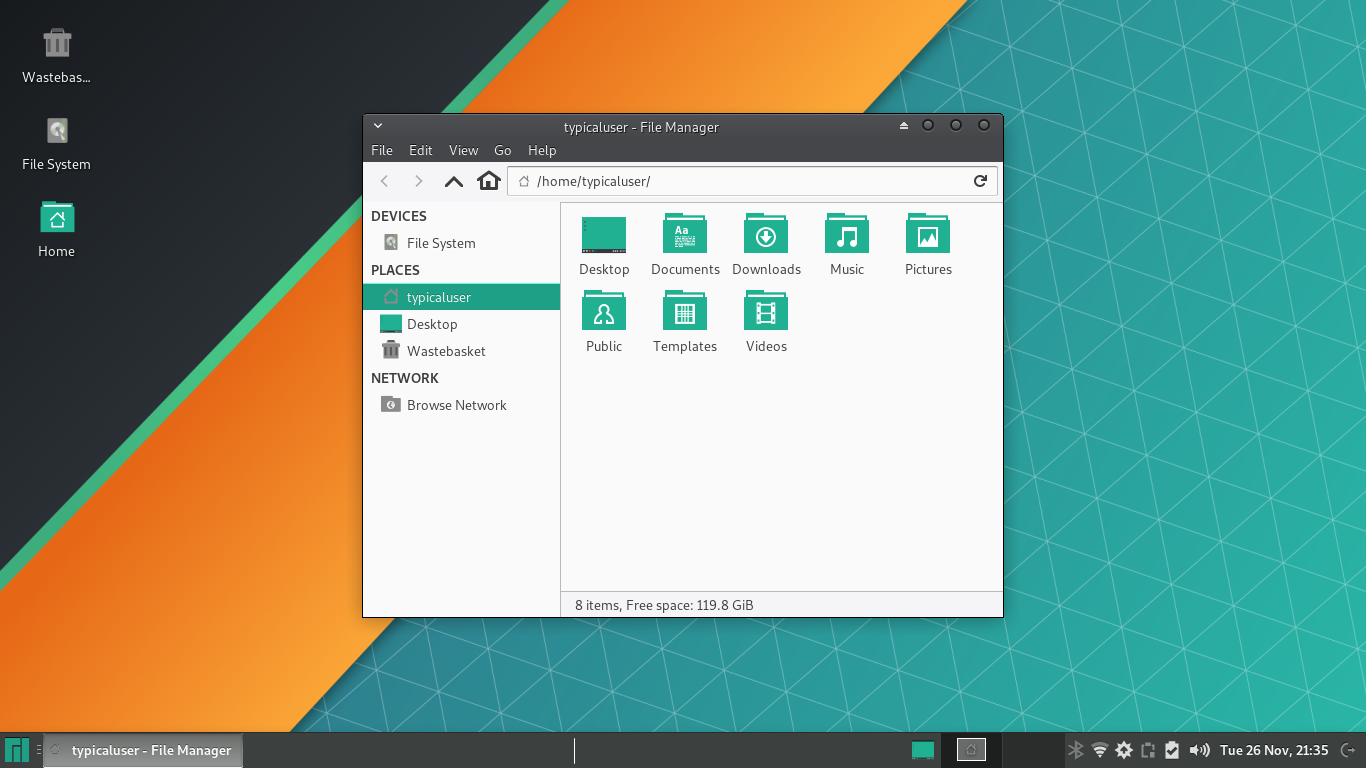
\includegraphics[scale = 0.25]{linuxthunar1.png} \hspace{1em}

花點時間確定你的最上層目錄。對於初學者來說,正確地做到這一點很重要。在 Windows 系統上,你應該使用檔案總管 \footnote{不要與 IE 瀏覽器混淆,後者是瀏覽器,與 Firefox、Chrome 和 Safari 執行相同的工作,你可能也知道並使用過。它們用於上網---也就是說,它們讓你可以存取遠端系統上的內容。檔案總管用於在本地 Windows 系統上儲存、查找和移動內容。要確保你知道這兩者之間的區別!},並且在 iOS(即 Apple 設備)上你應該使用 Finder。

再花點時間將你的最上層目錄與上圖進行比較。你可能是一個全螢幕,你可能是一個名稱列表而不是圖標,你可能沒有像左側那樣的面板。確保你可以找到當前目錄的名稱。在我的系統上,用戶的最上層目錄與該用戶具有相同的名稱。所以它是上圖中的``typicaluser''。

\newpage 現在看下圖,它顯示了 typicaluser 的圖片文件夾\footnote{也就是,圖片子目錄}的內容。

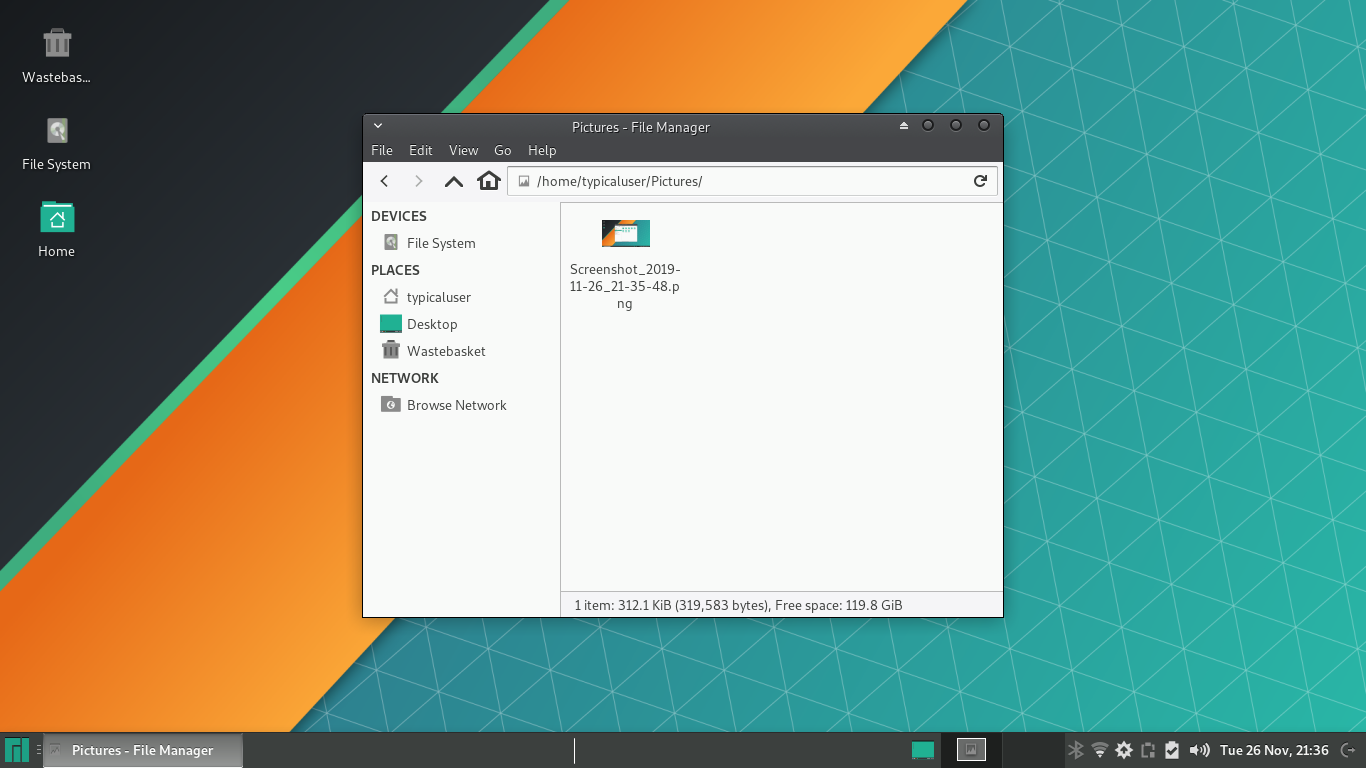
\includegraphics[scale = 0.25]{linuxthunar2.png}

現在文件夾的名稱只出現在一處。還要注意,在我的系統上,它給出的名稱不僅僅是``Pictures'',而是``/home/typicaluser/Pictures''。這被稱為提供完整路徑,它表示顯示的文件和/或子目錄包含在名為 Pictures 的文件夾中,該文件夾位於名為 typicaluser 的文件夾中,該文件夾位於名為 home 的文件夾中。

最後,如果這對你來說是全新的,請把玩\footnote{對大多數人來說最簡單的是使用滑鼠,但還有其他方法。但是,無論是單擊還是雙擊,是否可以拖放,是否可以使用多個按鈕等等,都取決於你的系統。}你的主目錄中的文件和文件夾。確保你可以從這個目錄移到另一個目錄,然後再返回。添加一個你自己輸入名稱的子文件夾,移到它(我也可以說``導航到它''),在這個新文件夾中創建一個文檔文件,重命名文檔文件,刪除文檔文件,移回 到你的用戶目錄,並刪除你的新文件夾。

現在移動到一個完全不同的文件夾,如果可能的話不在你的個人用戶目錄中。確保你可以找到文件夾的名稱並且你可以移回你的個人用戶目錄。

這是本課程的一個非常重要的時刻:當你啟動電腦時,預設情況下,你們中的大多數人都會是在你的個人用戶目錄中,這使得上面的練習相對容易,但這還不夠。你需要能夠確定你在目錄結構中的位置、你正在查看的文件夾的確切名稱以及如何移動到結構的其他部分。為此,你通常可以像在此處一樣使用文件夾管理系統,但有時你必須應用你對所需文件夾路徑的了解。

最後,現在或以後,創建一個專用於本課程的文件夾。在其中,你將儲存從課程網站下載的所有內容、你為課程編寫的所有代碼以及你可能希望添加的其他內容。我建議你通過創建一些子文件夾來組織一下,可能一個稱為 CourseMaterials 用於你的下載,另一個可能稱為 MyCodeAnswers 用於你為解答我們設置的任務而編寫的 Julia 代碼。

恭喜!你已經完成了為本課程設置你的系統的最重要和最棘手的部分。

\subsection*{寫入和儲存純文字文件}

(也稱為``純文字文件")

無疑的,你熟悉電腦上的文件準備系統。畢竟,編寫文檔是個人電腦最常見的用途之一。這些系統可以在本課程中使用,但不是很容易。使用 MS-Word 或 Pages 之類的東西,電腦付出很多努力讓你輕鬆編寫具有專業外觀的文檔。這意味著他們在後台做一些事情,比如設置段落縮排和分段、選擇漂亮的字體、設置可調整的邊界和表格等等。你會看到結果,但不會看到它是如何完成的。但是,儘管你沒有看到,但資訊必須在文件中,因此典型的 .docx 和 .pdf 等文件包含許多讀者甚至編寫文件的人都看不到的資訊。在某些系統中,你可以要求查看一些額外的內容(例如,在 MS-Word 中,你可以要求查看非打印字符)。

所有這些額外的資訊對 Julia 程式來說都是致命的。你將在本課程中看到 Julia 只能處理包含有效 Julia 代碼的程式,僅此而已。因此,文件系統以 .doc、.pdf 和其他專用格式放置的所有格式和其他資訊對 Julia 來說就像毒藥。你必須堅持這些額外資訊均不在你儲存且將運行的檔案中。也就是說,你編寫的檔案必須是純文字檔案。

我發現使用像 Mousepad 或 Notepad+ 這樣的程式最容易,它專門用於創建純文字檔案,僅此而已。假如以這種方式使用 MS-Word 或 LibreOffice 可能很困難。這些系統確實可以創建純文字檔案,但標準的方法是在第一次保存文件時選擇 .txt 副檔名。由於 Julia 程序使用 .jl 副檔名,這種方法通常意味著你首先使用 .txt 副檔名保存它,然後轉到你的文件夾管理系統並重命名它。

作為練習,轉到本課程的文件夾並創建一個純文字檔案。在其中寫一條短訊息,只使用純文字(即標準國際鍵盤上的羅馬字母,沒有重音、符號、中文或漢字)。使用標準的 .txt 副檔名儲存此檔案。現在更改檔案,仍然只使用標準的羅馬字母,並使用不同的副檔名保存它。使用不同的程式查看文件以確保它只包含你使用的字母、空格和標點符號,不多也不少(例如,在 MS-Word 中,以可見的非打印字符查看它)。最後,如果你有一個允許你這樣做的編輯器,則直接使用與 .txt 不同的副檔名創建一個純文字檔案。

\subsection*{啟動 Julia REPL}

當然,我們假設你的電腦上安裝了 Julia\footnote{可以線上運行 Julia,最顯易的是透過登錄 juliabox.com 在 JuliaBox 上運行,但在這種情況下,你無法按照所寫的方式完成課程。你當然可以查看課程材料,但是你需要的 Julia 練習將不會按照我們的計劃進行。在 JuliaBox 上,你沒有 REPL,而是專門的 IJulia 環境。這與 REPL 有細微差異但在重要的方面有所不同。如果你更喜歡在沒有安裝 Julia 的情況下使用它,並且你不介意我們提到的差異,請隨時繼續。}。所以啟動它---確切地如何啟動一個程式取決於你的系統,可能是一個單擊或雙擊圖標,或者是在一個特殊的視窗輸入``julia''並按 Enter 。如果一切順利,你會看到一個新視窗打開,看起來像這樣:

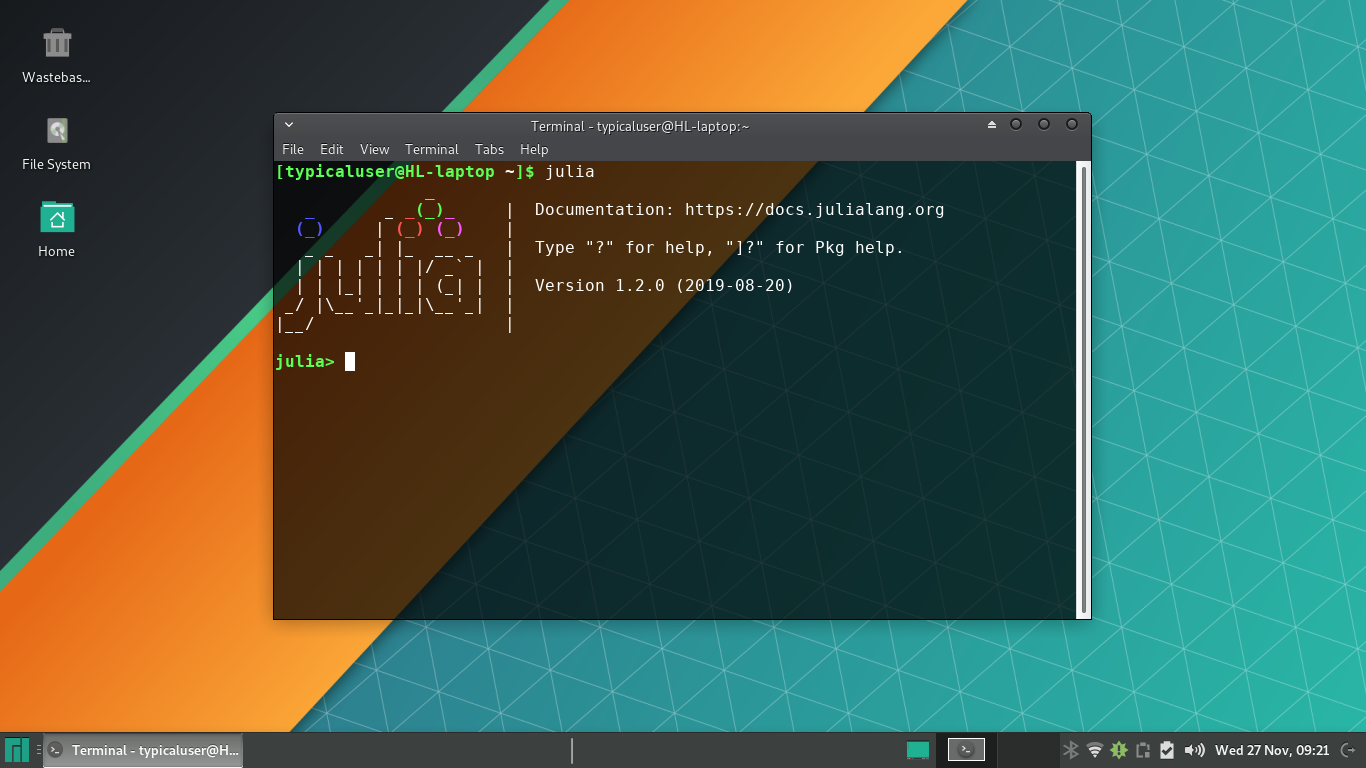
\includegraphics[scale=0.25]{REPL.png}

這是 Julia REPL。請注意,它以 Julia 正在運行的訊息和版本開頭,以及有關官方文件和幫助系統中更多資訊的一些提示。然後,在新的一行上顯示文字 {\tt julia$ > $}。這是 Julia 提示,如果你在此視窗中輸入(你可能必須先單擊它),你應該會看到你輸入的內容出現在提示的右側。你將在本課程中進行大量此類輸入。完成輸入後,你通常會按 Enter,並且(也許一段時間後,可能會在你的電腦上發生一些可見到或可聽到的事情),你將再次看到 {\tt julia$ > $},等待你輸入更多 Julia 代碼。

要結束你的 REPL 會話,只需按 Ctrl-D(即按住鍵盤上的 Ctrl 按鈕並按 D 鍵,不必將其設為大寫字母,但也沒有任何區別)。或者,鍵入 \codequote{exit()} 並按 Enter。

\section*{關於如何完成本課程的簡要建議}

正如我們在第 1 週的第 4 課中所堅持的那樣,Julia 是一種語言:學習語言的測試是用它來表達自己。在程式設計的情況下,當你表達自己並運行你的程式時,電腦最終會做一些事情:它創建和顯示文字、繪製圖形、計算數字、在紙上列印東西、播放聲音等。

如果不練習表達自己,你就無法學會表達自己。所以主要的建議是:編寫大量的 Julia 表達式,看看當你嘗試運行生成的代碼時會發生什麼。如果你收到錯誤訊息,請不要擔心。相反的,請利用錯誤訊息(這包括忽略那些不重要的訊息)。

當然,跟著課程。但要能中斷,在 REPL 和 {\tt .jl} 檔案中嘗試一下。回顧你不確定的事情。關鍵是要保持活躍,而不是僅僅跟隨教材而陷入困境。

練習和評估也很重要,因為它們可以幫助你了解你已經走了多遠以及你是否準備好繼續。他們給你反饋---但最重要的反饋來源仍然是 REPL 本身。Julia 語言本身會教你如何使用它---你所要做的就是繼續和它對話。在這方面,它與學習任何其他語言沒有太大區別。

\section*{課程內容}
這裡是課程內容的總結(濃縮的,僅粗略按出現順序)

--- 字串文字\\
--- 名稱(包括保留字)\\
--- 變數 \\
--- 函數 \\
--- 從 REPL 運行 Julia 代碼檔案 \\
--- 除錯 \\
--- 每種電腦語言的規則都是嚴格的,因為每種電腦語言都是通過形式邏輯構建的,但是 \\
--- 一個人不需要知道形式邏輯來學習如何撰寫程式 \\
--- 表達式(它們由值、名稱、分隔符號和運算子組成;Julia 代碼的每一塊都必須是有效的表達式)\\
--- 字串運算子、比較運算子、邏輯運算符 \\
--- 資料容器(字串和一維陣列)\\
--- 算術 \\
--- 類型系統和多重派遣 \\
--- 範圍 \\
--- 結構(特別是由關鍵字 \codequote{if}、\codequote{while} 和 \codequote{for} 引入的結構)\\

這為你將 Julia 用於非常有趣的專案奠定了基礎,正如我們在第 4 週的課程中所展示的那樣。當然,它仍遺漏了 Julia 語言的許多特別之處。在本課程的最後一課中,我們將簡要討論 Julia 的內容比本課程涵蓋的內容多出多少。我們還為你提供了繼續程式設計冒險的方法---我們希望是在 Julia,但不堅持是它!

\end{document}
